%% Do not edit unless you really know what you are doing.
\documentclass[12pt,a4paper]{report}
\usepackage[T1]{fontenc}
\usepackage[latin1]{inputenc}
\usepackage{color,geometry,graphicx}
\usepackage[absolute]{textpos}
\usepackage{doxygen}
\usepackage{pdfpages}
\usepackage{float,textcomp,amsmath,paralist,calc}
\usepackage{natbib}
\usepackage{titlesec}
\usepackage{xr}
\usepackage[titletoc]{appendix}
\geometry{verbose,a4paper,tmargin=1in,bmargin=1in,lmargin=1in,rmargin=1in}
\newcommand{\ap}{\textquotesingle}
\newcommand{\sq}[1]{\textquotesingle{#1}\textquotesingle}
\setlength\parindent{0pt}

% from Doxygen refman.tex------------------------------------------------------
\usepackage{sectsty}
\renewcommand{\familydefault}{\sfdefault}
\allsectionsfont{%
  \fontseries{bc}\selectfont%
  \color{darkgray}%
}
\renewcommand{\DoxyLabelFont}{%
  \fontseries{bc}\selectfont%
  \color{darkgray}%
}
\newcommand{\+}{\discretionary{\mbox{\scriptsize$\hookleftarrow$}}{}{}}
% from Doxygen refman.tex------------------------------------------------------

\definecolor{gray}{rgb}{0.8,0.8,0.8}

\newcommand{\frontmatter}{\cleardoublepage
  \pagenumbering{roman}}
\newcommand{\mainmatter}{\cleardoublepage
  \pagenumbering{arabic}}
\newcommand{\backmatter}{\cleardoublepage}

%%%%%%%%%%%%%%%%%%%%%%%%%%%%%% User specified LaTeX commands.
%\renewcommand{\baselinestretch}{1.5}

% hyperlinks to sections and references
\usepackage{cite}
\usepackage{hyperref}
\hypersetup{colorlinks, linkcolor=blue, citecolor=blue, urlcolor=blue}
%\usepackage[pdftex,bookmarks=true,bookmarksnumbered=true,pdfpagemode=None,pdfstartview=FitH,pdfpagelayout=SinglePage,pdfborder={0 0 0}]{hyperref}
\newcommand{\tsup}[1]{\textsuperscript{#1}}
\newenvironment{desclist}[1]
{\begin{list}{}
{\renewcommand\makelabel[1]{{##1}\hfill}
\settowidth\labelwidth{\makelabel{#1}}
\setlength\leftmargin{\labelwidth+\labelsep}}}
{\end{list}}

\newenvironment{adescription}[1]
{\begin{list}{}
{\renewcommand\makelabel[1]{\texttt{##1}\hfill}
\settowidth\labelwidth{\makelabel{#1}}
\setlength\leftmargin{\labelwidth+\labelsep}}}
{\end{list}}

% Package name and version
\def\pack{MeshAssist}
\def\packver{\pack\ v1.0.0}

\begin{document}
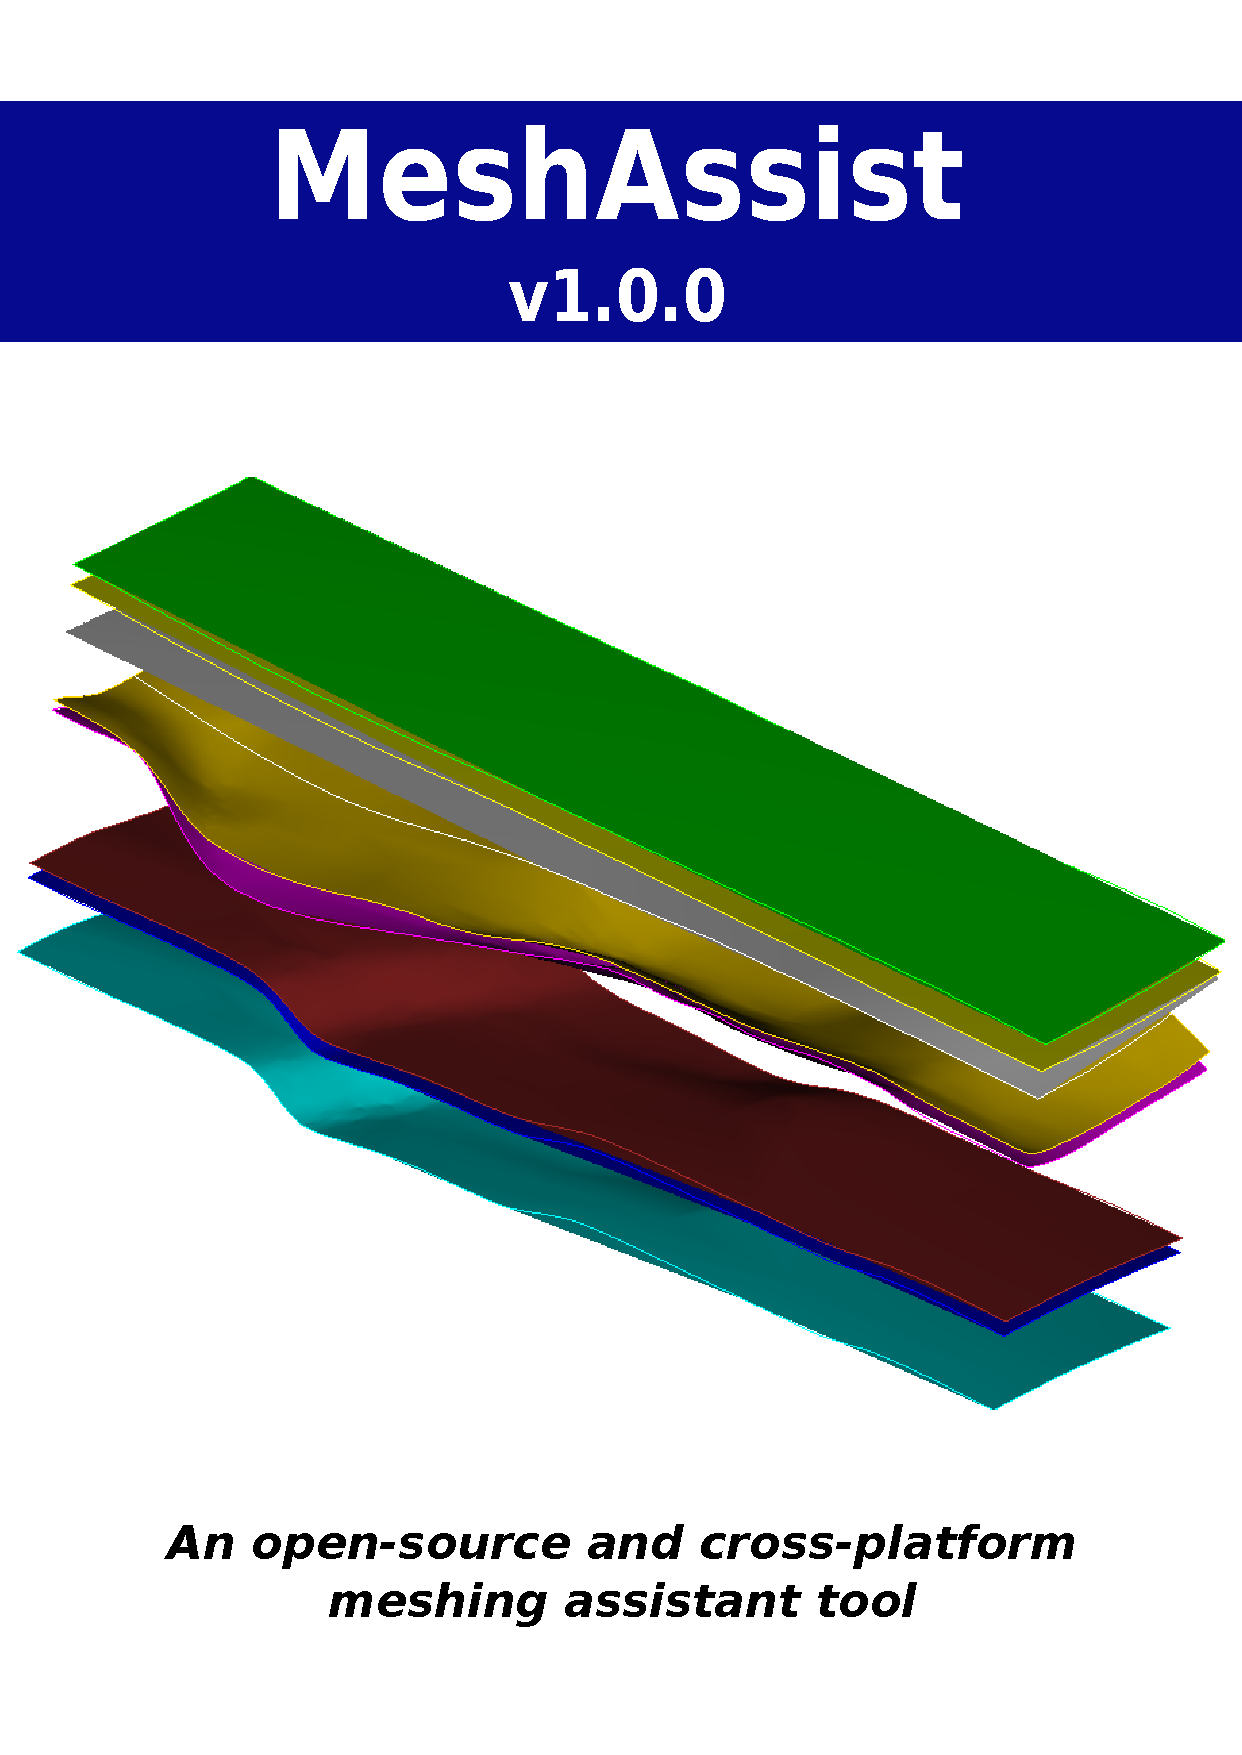
\includepdf[fitpaper]{cover_MeshAssist}

\thispagestyle{empty} % no page number
\title{\textbf{\packver \\
User Manual}}

\author{
Hom Nath Gharti\footnote{formerly at: NORSAR, Norway; and Institute of Engineering, Tribhuvan University, Nepal}, Princeton University, USA \\
Leah Langer, Princeton University, USA \\
Michael Roth, NORSAR, Norway \\
Jeroen Tromp, Princeton University, USA \\
Uno Vaaland, Princeton University, USA \\
Zhenzhen Yan, Institute of Remote Sensing and Digital Earth, CAS, China
}


\maketitle

\frontmatter

\addcontentsline{toc}{chapter}{Licensing}
\chapter*{Licensing}
%
%\packver\ \\
%Copyright 2017 Hom Nath Gharti\\
%
%This file is part of \packver.\\
%
\packver\ is free software: you can redistribute it and/or modify
it under the terms of the GNU General Public License as published by
the Free Software Foundation, either version 3 of the License, or
(at your option) any later version.\\

\packver\ is distributed in the hope that it will be useful,
but WITHOUT ANY WARRANTY; without even the implied warranty of
MERCHANTABILITY or FITNESS FOR A PARTICULAR PURPOSE.  See the
GNU General Public License for more details.\\

You should have received a copy of the GNU General Public License 3.0
along with \linebreak\packver.  If not, see <\texttt{http://www.gnu.org/licenses/}>.\\

\clearpage

\addcontentsline{toc}{chapter}{Acknowledgments}
\chapter*{Acknowledgments}
 Part of this document was prepared by using the documentation generator "Doxygen" (Main developer: Dimitri van Heesch) and the Matlab parser for Doxygen "doxymatlab" (Main developer: Fabrice).

\clearpage

\tableofcontents
\clearpage

\mainmatter
\chapter{Introduction}
\label{chap:intro}
\section{Background}

 \pack\ is a collection of tools which assists meshing of complex and 
 realistic 2D/3D models for FEM/SPECFEM simulations. As its name suggests,
 it is NOT a meshing software. It is only a meshing assistant!

\section{Cite as}
Gharti, H. N.; Langer, L.; Roth, M.; Tromp, J.; Vaaland, U.; Yan, Z. (2017). MeshAssist: an open-source and cross-platform meshing assistant tool. Zenodo. http://doi.org/10.5281/zenodo.883448

\section{Status summary}
\begin{desclist}{Digital Elevation Model (DEM)} % put logenst string in {}
\item[Digital Elevation Model (DEM)]        : Yes
\item[DXF AUTOCAD Model]        : Yes
\item[GOCAD Model]        : Yes
\item[EXODUS mesh]        : Yes
\item[GiD mesh]        : Yes
\item[VTK file]        : Yes
\item[VTU file]        : Yes
\item[XYZ file]        : Yes
\end{desclist}

\section{Changes made since the last version}
\begin{itemize}
\item This is the first version.
\end{itemize}

\chapter{Getting started}
\label{chap:start}
\section{Package structure}
The \pack\ pacakge can be obtained using Git. Use the following command in the terminal:\\

\texttt{git clone \-\-recursive https://github.com/homnath/MeshAssist.git}\\

The package has the following structure:\\

\texttt{\pack/}
\begin{adescription}{~~CMakeLists.txt}
\item[~~LICENSE]               : License.
\item[~~Makefile]                : brief description of the package.
\item[~~bin/]                  : all object files and executables are stored in this folder.
\item[~~doc/]                  : documentation file/s for the \pack\ package.
\item[~~input/]                : contains input files.
\item[~~output/]               : default output folder. All output files are stored in this folder unless the different output path is defined from command.
\item[~~src/]                  : contains all source files.
\end{adescription}
 
\section{Prerequisites}

The package requires Make utility, latest C and Fortran compilers. For matlab files, Matlab is necessary.

\section{Configuration}

Open src/Makefile and modify the C and Fortran compilers if necessary.

\section{Compile}

Type the following command in the terminal

make all

Matlab files can be opened in and run from Matlab.

\section{Run}

{\em command} {\em input\_file} [{\em Options}]

Example:

./bin/xyz2jou ./input/xyz2jou\_example.utm

See Chapter "File Documentation" for all available commands. 

\section{Bug Report}

hgharti\_AT\_princeton\_DOT\_edu

\chapter{File Index}
\label{chap:files}
\input{./latex/files.tex}

\chapter{File Documentation}
\label{chap:filedoc}
\input{./latex/dem2vti_8m.tex}
\newpage
\input{./latex/dxf2jou_8m.tex}
\newpage
\input{./latex/dxf2jou__vertex_8m.tex}
\newpage
\input{./latex/exodus2semgeotech_8c.tex}
\newpage
\input{./latex/exodus2specfem2d_8c.tex}
\newpage
\input{./latex/exodus2specfem3d_8c.tex}
\newpage
\input{./latex/exodusold2semgeotech_8c.tex}
\newpage
\input{./latex/exodusold2specfem3d_8c.tex}
\newpage
\input{./latex/gid2semgeotech_8c.tex}
\newpage
\input{./latex/gocad2vtu_8c.tex}
\newpage
\input{./latex/vti2cell_8c.tex}
\newpage
\input{./latex/vtk1d2jou_8f90.tex}
\newpage
\input{./latex/vtk2d2jou_8c.tex}
\newpage
\input{./latex/write__vti_8m.tex}
\newpage
\input{./latex/xyz2jou_8f90.tex}


%\begin{appendices}
%  \input{a1_cubit_example}
%\end{appendices}

\bibliographystyle{chicago}
\bibliography{manual_MeshAssist}

\end{document}
